\documentclass[../main.tex]{subfiles}

\begin{document}

\chapter{June $27^{th} / 2025$}
\label{ch:tufte-design}

\section{AlphaGenome: advancing regulatory variant
effect prediction with a unified DNA sequence
model}\cite{Avsec2024AlphaGenome}

\textbf{Challenge}: Interpretation of non-coding genetic variants - 98\% of human genetic variation and difficult to understand due to diverse / subtle effects on gene regulation.

\vspace{0.3cm}

\textbf{Trade-off} between \textit{length} and \textit{prediction resolution} due to computational limitations

\begin{itemize}
    \item \textbf{High Resolution, short sequence length:}Some models (e.g., BPNet, SpliceAI) achieve high nucleotide-level predictive resolution at the \textbf{cost} of being restricted to short input DNA sequences 10kb or less. \textbf{CANNOT} capture long-range genomic interactions and miss influence of important distal regulatory elements that lie outside limited input window
    \item \textbf{Long Sequence Length, low resolution:} Models like \textbf{Enformer} and \textbf{Borzoi} can process long DNA seq. ($\approx200kb$ to $\approx500kb$), which allows them to capture a broader regulatory context. The trade-off is resolution of predictions must be reduced (e.g., group output into bins of 32 or 128 bps). May miss blur fine features
\end{itemize}

$\bullet$ \textbf{Multimodal Predictions}: Prediction Ks genomic features across $11$ different modalities (RNA-seq, CAGE), chromatin accessibility (ATAC-seq, DNase-seq), histone modifications, transcription factor binding, chromatin contact maps (Hi-C) and detailed splicing patterns (splice, usage, junctions)

\vspace{0.3cm}

$\bullet$ \textbf{Splicing:} First model to predict splices sites, splice site usage, and splice junctions counts simultaneously $\rightarrow$ How do variants disrupt splicing?

\vspace{0.3cm}

$\bullet$ Foundation of AlphaGenome is vast / diverse collection of public functional genomics data from human (hg38 reference genome) and mouse (mm10 reference genome) sources. Process was standardized to ensure high quality and consistency.

\begin{itemize}
    \item \textbf{Data Sources and Standardization}
    \begin{itemize}
        \item Aggregation from ENCODE, FANTOM5, GTEx:
        \begin{itemize}
            \item RNA-seq, CAGE, PRO-cap, DNase-seq, ATAC-seq, ChIP-seq, chromatin contact maps
        \end{itemize}
        \item Standardize metadata for ALL samples:
        \begin{itemize}
            \item UBERON for tissues, EFO/CLO for cell lines, CL for primary cell types
        \end{itemize}
        \item QC step for all ENCODE $=$ application of ENCODE's audit system
    \end{itemize}
\end{itemize}



\subsection{Processing of Specific Data Types} (More specific)

\textbf{RNA-seq}

\begin{itemize}
    \item Data from both ENCODE and GTEx (via RECOUNT3) were used.
    \item To ensure comparability, all tracks were normalized to Reads Per Million (RPM) and then further rescaled to a common factor of 100 million total reads.
    \item Tracks were then grouped by biological context (ontology term, assay type, etc.) and averaged to create final representative tracks for model training.
\end{itemize}

\textbf{CAGE and PRO-cap}

\begin{itemize}
    \item CAGE data from FANTOM5 and PRO-cap data from ENCODE were processed similarly to RNA-seq, with individual tracks normalized to a total of 100 million reads before any averaging.
\end{itemize}

\textbf{DNase-seq and ATAC-seq (Chromatin Accessibility)}

\begin{itemize}
    \item Instead of using pre-processed signal files, raw alignment (BAM) files were used to preserve base-resolution information.
    \item These were converted to bigWig files that record the counts of enzyme cut sites at each base.
    \item This approach allows for the correction of enzyme cut bias by applying appropriate read shifts ($+4/-4$ for ATAC-seq and $0/+1$ for DNase-seq).
    \item The resulting tracks were averaged within ontology groups and normalized to 100 million insertions per track.
\end{itemize}

\textbf{ChIP-seq (TF and Histone)}

\begin{itemize}
    \item Only "fold change over control" signal files were selected.
    \item After stringent QC and hierarchical filtering to select the most representative experiments, the fold-change signals were averaged within each biological context group without further normalization.
\end{itemize}

\textbf{Splicing Data (Junctions, Sites, Usage)}

\begin{itemize}
    \item RNA-seq reads were realigned using STAR to specifically detect and quantify splice junctions.
    \item \textbf{Splice Junctions}: Raw junction counts were subjected to a stringent quality filtering pipeline to ensure high confidence. The retained counts were then normalized and scaled for model training.
    \item \textbf{Splice Site Usage (SSU)}: SSU was calculated for each potential splice site. The quantification was performed considering all reads spanning the splice sites regardless of the strand. The formula used is:
    \begin{equation}
        \text{SSU} = \frac{\text{\#reads using the splice site}}{\text{\#reads using the splice site} + \text{\#reads supporting skipping of the splice site}}
    \end{equation}
    \item \textbf{Splice Site Classification}: The set of all unique donor and acceptor sites from the filtered junction data was used to define the training examples for a 5-class classification task (Donor+, Acceptor+, Donor-, Acceptor-, or Not a splice site).
\end{itemize}

\textbf{Contact Maps}

\begin{itemize}
    \item Hi-C and Micro-C datasets were sourced from the 4D Nucleome portal.
    \item The maps were processed following the Orca protocol, which includes matrix balancing and adaptive coarse-graining.
    \item A distance-based normalization was applied to compute a log-fold change over the average contact value for each genomic distance. The normalized contact map values $y_{i,j}$ were computed as:
    \begin{equation}
        y_{i,j} = \log\left(\frac{x_{i,j} + \epsilon}{\text{mean}[|i-j|] + \epsilon}\right)
    \end{equation}
    where $x_{i,j}$ is the coarse-grained count, $\epsilon$ is a numerical relaxation constant, and $\text{mean}[|i-j|]$ is the average coarse-grained contact value for the pairwise genomic distance.
\end{itemize}






\vspace{0.3cm}

\subsection{Splicing}

Process that generates mature mRNA sequences. It functions by removing non-coding regions (\textbf{introns}) and joining remaining coding regions  (\textbf{exons}) 

\vspace{0.3cm}

\begin{center}
    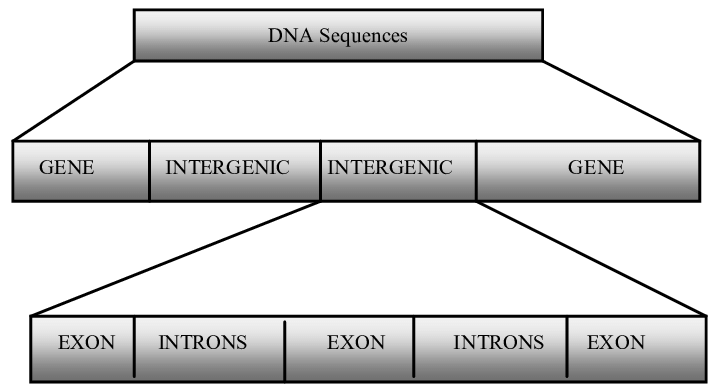
\includegraphics[width=8cm]{files/images/dna_intronexon.png}    
\end{center}

Genetic variants may disrupt splicing which alters final mRNA $\rightarrow$ aberrant protein 

\vspace{0.2cm}

\begin{itemize}
    \item \textbf{Splice Sites}: Specific nucleotides in DNA seq. that signal where splicing machinery should \textit{cut and join} RNA. They mark boundaries between introns and exons: 
    \begin{itemize}
        \item \textbf{Splice Donors:} beggining of intron 
        \item \textbf{Splice acceptor:} End of intron 
    \end{itemize}

    Probability any given nucleotide will function as donor / acceptor can be modeled and such sites are associated with \textit{recognizable sequence motifs}. \textbf{$\alpha$Genome} predicts classification of these sites on \textbf{positive} and \textbf{negative} DNA strands (wtf is this?)
\end{itemize}

\subsection{Splice Junction}
Specific connection point where $2$ exons are ligated (joined) together after having intron excised. Prediction of which introns are removed $=$ \textbf{Splice Junction Prediction}

\begin{figure}[h!]
    \centering
    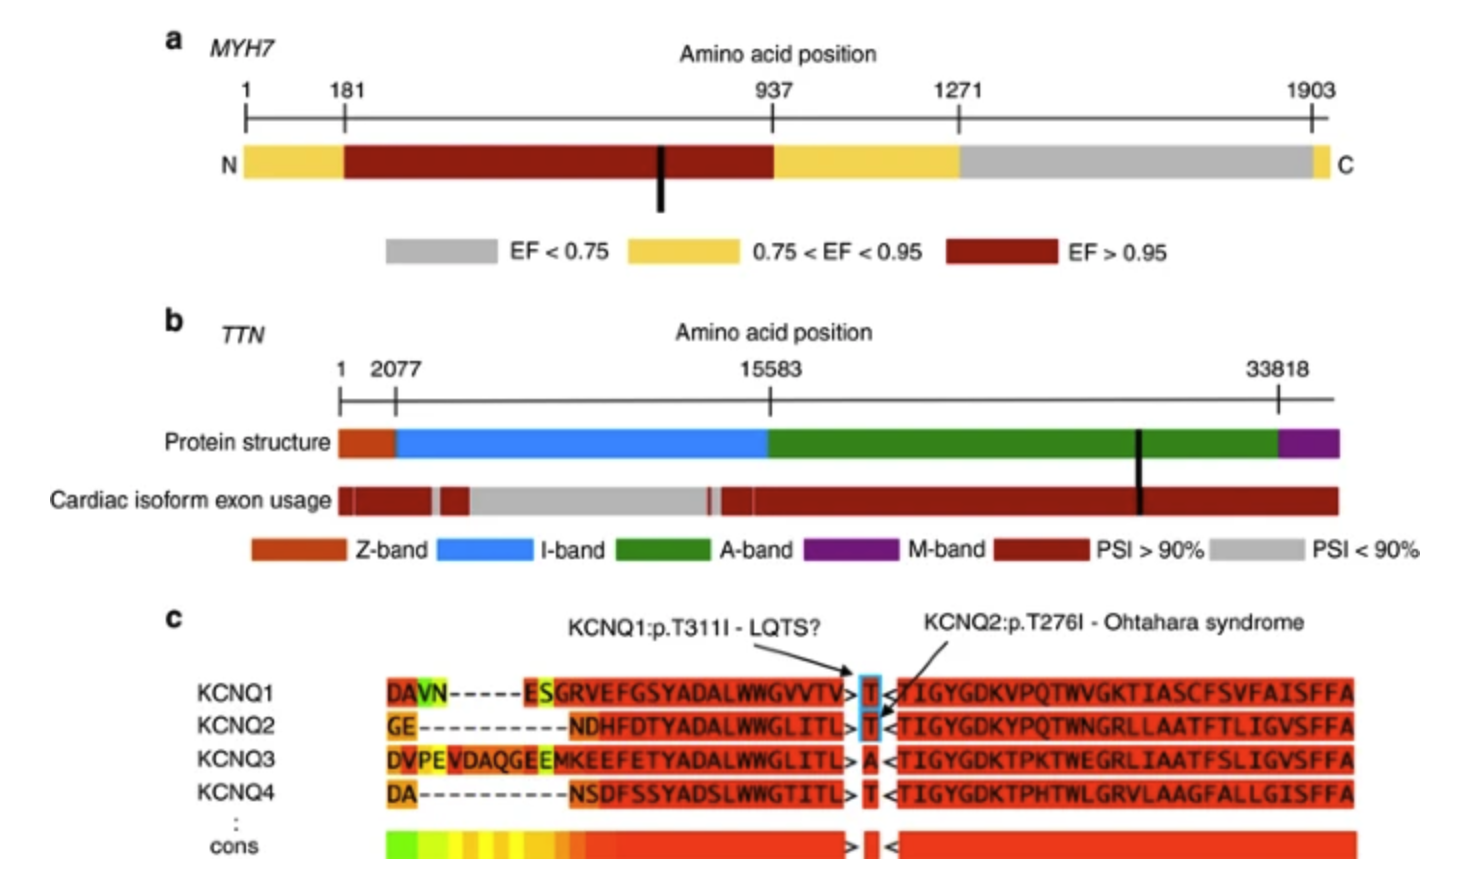
\includegraphics[width=12cm]{files/images/disease_specific.png}
    \caption{(a) Missense variants within a subportion of \textit{MYH7}, when identified in an HCM patient, have a 97\% prior probability of being pathogenic (etiological fraction; EF $=$ 0.97). We activate PM1 for missense variants in this region. Here we use \textit{MYH7:c.2221G>T} as an example (black bar). (b) Truncating variants in \textit{TTN} are only known to cause DCM when found in exons constitutively expressed in the heart (proportion spliced in $>$0.9). We activate PVS1\_strong for these variants. Here we use \textit{TTN:c.86641delC} as an example (black bar). (c) Variants that have been identified as pathogenic in paralogous genes may identify residues that are intolerant to variation. We have created two modified rules, PS1\_moderate and PM5\_supporting, to incorporate this evidence. Here we use \textit{KCNQ1:p.T311I} as an example. \textit{KCNQ2:p.T276I} is associated with Ohtahara syndrome. We activate PS1\_moderate for \textit{KCNQ1:p.T311I}, which is the equivalent missense change (i.e., same reference and alternate amino acids) in a different member of the same protein family.}
\end{figure}

\begin{tikzpicture}[
    node distance=1.5cm and 2cm,
    block/.style={rectangle, draw, fill=blue!10, text width=8em, text centered, rounded corners, minimum height=4em},
    io/.style={trapezium, trapezium left angle=70, trapezium right angle=110, draw, fill=green!10, text width=8em, text centered, minimum height=4em},
    decision/.style={diamond, draw, fill=orange!10, text width=6em, text centered, aspect=1.5},
    line/.style={draw, -{Stealth[length=2mm]}},
    label/.style={font=\scriptsize\itshape}
]

% Nodes
\node[io] (input) {Patient Whole-Genome Data \& VUS List};

\node[block, below=of input] (alphagenome) {AlphaGenome Core Processing};
\node[label, right=0.1cm of alphagenome, text width=12em, align=left, anchor=west] {A single model pass generates scores for each VUS across all modalities.};

\node[block, below left=of alphagenome] (splicing) {Splicing Disruption Analysis};
\node[block, below=of alphagenome] (expression) {Regulatory Impact Analysis (e.g., eQTLs)};
\node[block, below right=of alphagenome] (ism) {Mechanistic Analysis (ISM)};

\node[decision, below=2cm of expression] (integrate) {Integrate Functional Evidence};

\node[io, below=of integrate, trapezium angle=80] (output) {Prioritized Candidate Variants for Clinical Review};

% Faded box for AlphaGenome outputs
\node[draw=gray, dashed, inner sep=0.5cm, fit=(splicing) (expression) (ism), label={[gray]above:Multimodal Outputs}] (outputs_box) {};

% Arrows and Labels
\path [line] (input) -- (alphagenome);
\path [line] (alphagenome) -- node[label, left, pos=0.4] {Splicing Scores} (splicing);
\path [line] (alphagenome) -- node[label, left] {Expression Scores} (expression);
\path [line] (alphagenome) -- node[label, right, pos=0.4] {Contribution Scores} (ism);

\path [line] (splicing) -- (integrate);
\path [line] (expression) -- (integrate);
\path [line] (ism) -- (integrate);

\path [line] (integrate) -- (output);


\end{tikzpicture}


\end{document}